\documentclass[12pt,a4paper,final,oneside]{report}
\usepackage{graphics}
\usepackage{graphicx}
\usepackage{txfonts}
\usepackage{float}
\paperheight 297mm
\paperwidth 210mm
\topmargin 15mm
%\bottommargin 22mm
\footskip 11mm
\oddsidemargin 20mm
\evensidemargin 20mm
\setlength{\textheight}{9.5in}%9.5in
\setlength{\textwidth}{6.3in} %6.3in
\begin{document}
\begin{center}
A Project Report On\\
\LARGE{SpielPlatz}
\end{center}
\vspace{2cm}
\begin{center}
Submitted in partial fulfilment for the
\linebreak Degree of \textbf{Bachelor of Engineering} in
\linebreak Computer Science and Engineering
\end{center}
\vspace{1cm}
\begin{center}
Submitted by 

\textbf{BHAVIKA PATEL(140060107007)}\\
\textbf{RAHUL RATHI(140060107046)}\\
\textbf{DIVYA LIMBANI(12006013)}\\
\textbf{BANDRE MAYURI(140063131005)}\\
\vspace{1cm}

Under the Guidance of 
\linebreak \textbf{MR.KRUNAL PATEL} \linebreak
\textbf{MRS AMI PATEL}
\end{center}

%-------------------------------------------------
%\centering
	\begin{figure}[h]
		\centering
		\includegraphics[width=0.35\linewidth,angle=0]
		{bm.jpg}
		
	\end{figure}
%---------------------------------------------------------
\vspace{0.7cm}
\begin{center}
\textbf{Department of Computer Science and Engineering\\
Bhagwan Mahavir College of Engineering and Technology,}
\linebreak Bharathana-Vesu, Surat -395017.
\linebreak Gujrat Technological University
\linebreak September, 2017
\end{center}

\newpage
\thispagestyle{empty}
\begin{center}
		\LARGE{CERTIFICATE}
\end{center}
	
	
\vspace{2cm}
	
	This is to certify that Bhavika Patel (140060107007), Rahul Rathi (140060107046), Divya Limbani(140060107005), Mayuri Bandre(140060107058) have completed the project report on the topic "SpielPlatz" satisfactorily in partial fulfilment for the Bachelor's Degree in Computer Science and Engineering under the guidance of Mrs.Ami Patel during the year 2016-17 as prescribed by Gujarat Technological University.
	
\vspace{3cm}
	
	\begin{flushleft}
Guide \hfill Head of the Department\newline
		
		
		
		Mrs. Ami Patel \hfill Mr. Krunal Patel
	\end{flushleft}
	
	
	
	\vspace{2cm}
	\begin{center}
		Principal
		
		
		
		Dr. Rajendra R. Sawant
	\end{center}
	
	\vspace{2cm}
	\begin{flushleft}
		Examiner 1 \hfill Examiner 2
	\end{flushleft}
\newpage
\begin{abstract}
\par The virtual environment for practising cyber security is indeed not only to the cyber security experts it will also be use full for the students , professional \&
the institution which preparing the next worriers . The virtual cyber lab includes the creation of labs ,sharing of  expensive hardware and tools . This lab not 
only focus on practical hands on practice but also on theatrical concepts and discussion  This lab is based on cloud arch and available over internet using just a
web browser. This lab also provide the GUI \& SSH connectivity over web and the lab is compatible with any device which has a HTML% supported web browser and a 
internet connection. There are available test bed's offered by various vendors like Cloud share , Breaking Point by IXIA (Cyber Range), Cybergym by an Israeli company
which offers the labs .We have vision of a virtual lab in which attacking team / individual who carries a cyber attack and the infrastructure for the attacks but the 
control is maintain by training expert or the individual who is practising.There is one more concert that the security of the cyber attack or practice should be 
walled inside the cloud practice environment.


\end{abstract}

\newpage
	
	\pagestyle{plain}
	\tableofcontents
	\listoffigures
	\chapter{Introduction}
	\noindent\textbf{}
	
	\section{ Problem Summary and Introduction:}
	
\noindent\textbf{} 
%	\justifying
\par In today's world cyber security is one of the major concern . The world of cyber security  attracting young talents for research , exploit \& defend for benefits . The young talents require training \& the formal fundamentals of the cyber security which leads to the major problem . The problems of cost , availability \& respective skills are more expensive than cyber security learning. Not only the cost of Practice comes in consideration , there some information security bodies which forces the law \& restriction for people good but they are interfering with the good practice of cyber security.
	%\justifying
	\raggedright
	\section{ Aim and objectives of the project:}
	%\justifying
	Our aim is to make a solution that not only provide the practice grounds but also the environment where people can collaborate on same interests . some research companies can make the profiles \& can use expensive resource on usage bases. We are also considering the LAW of information security in our concern.
	
	\noindent\textbf{}
	\noindent\textbf{}
	\newpage
	\section{ Problem Specifications :}
	%\justifying
\noindent\par The virtual environment for practising cyber security is indeed not only to the cyber security experts it will also be use full for the students , professional \& the institution which preparing the next worriers . The virtual cyber lab includes the creation of labs , sharing of  expensive hardware and tools . This lab not only focus on practical hands on practice but also on theatrical concepts and discussion.The problem specified comes for over head of vm environment they require powerful hardware which is costly and the running , maintaining cost id a overhead which can not be ignored.
	\section{ Brief literature review and Prior Art Search(PAS) about the project :}
	
	\noindent \textbf{}
	
	%\justifying
	\noindent\par 1. Java Core | Solution building \newline
2. Java advance | Solution Delivery \newline
3. Linux Fundamentals | Platform Fundamentals \newline
4. Cisco Inter-networking | Inter-networking

\noindent\textbf{} 
	
	\section{Plan of work :}
	
	\noindent 
		
	\noindent\textbf{}	
	\centering
	\begin{tabular}{|p{0.7in}|p{2.0in}|p{1.2in}|p{1.5in}|} \hline 
		\textbf{Sr. No.}\newline  & \textbf{Task}\newline  & \textbf{Estimated Day}\newline & \textbf{Comment}\newline  \\ \hline 
		\centering1 \newline & Understanding of JAVA \newline  & July\newline & N/A \newline \\ \hline 
		\centering2 \newline  \\ & Understanding of Platforms
		\newline  & August \newline & Linux \newline \\ \hline 
		\centering3 \newline  & Understanding of Delivery Mechanism
		\newline  & September \newline  & Tomcat \& Guacamole\newline  \\ \hline 
		\centering4 \newline  & Code Initialization \& Code Management
\newline  & October \newline \newline  & Git lab \& Code Prototype\newline  \\ \hline 
		\centering5 \newline \newline  & Submitted PPR and PSAR report and verify the documentation.
		\newline \newline  & October-November\newline & N/A \newline \newline  \\ \hline 
		\centering6 \newline  & Intensive logice design \& arguments \& Alternative \newline  & November \newline  & Database \newline  \\ \hline 
		\centering7 \newline  & Intensive Code \newline  & December\newline  & N/A \newline   \\ \hline 
		\centering8 \newline  & | Intensive test 
		\newline  & January \newline  & Plagiarism \newline  \\ \hline 
		\centering9 \newline  & Product validation
		\newline  & February \newline  & Learning \newline  \\ \hline 
		\centering10 \newline  & Costumer Validation \newline  & March\newline  & N/A\newline  \\ \hline 
	\centering11 \newline  & Closing , summary \& Business Profit Summary \newline  & March\newline  & N/A\newline  \\ \hline	
	\end{tabular}
	\noindent \textbf{}
	
	\centering
	Table 1: Project Plan 
	\noindent \textbf{}
	
	\newpage
	\raggedright
	\section{Materials/Tools required :}
	\noindent\textbf{}
	
	
	\subsection{Software Requirements :}
	
	\textbf{  }To run an application user need:\\
	\centering
	\noindent\textbf{} 
	
	\noindent\textbf{}
	Table 2:  Software need to run an application
	\noindent\textbf{} 
	
	\begin{tabular}{|p{0.7in}|p{2.4in}|p{2.1in}|} \hline 
		\textbf{Sr. No.}\newline  & \textbf{Name}\newline  & \textbf{Compatibility}\ \newline \\\hline 
		\centering1 \newline & Tomcat \newline  & Windows / mac / Linux\newline \\ \hline 
		\centering2 \newline & Guacamole Server \newline  & Linux\newline \\ \hline 
		\centering3 \newline & Fire-fox / chrome / safari  \newline  &  Appropriate Selection\newline \\ \hline 
	\end{tabular}
	\noindent\textbf{}
	\noindent\textbf{}
	
	
	\noindent\textbf{}
	\raggedright
	\subsection{Hardware Requirements :}
	\noindent\par To develop an application we need :\\
	\noindent\textbf{}
	\noindent\textbf{}
	\\
	\centering
	\noindent\textbf{}
	Table 2:Hardware ware need to run an application
	\noindent\textbf{} 
	
	\begin{tabular}{|p{0.7in}|p{2.4in}|p{2.1in}|} \hline 
		\textbf{Sr. No.}\newline  & \textbf{Name}\newline  & \textbf{Compatibility}\ \newline \\\hline 
		\centering1 \newline & PC \newline  & Windows / mac / Linux \& Virtualization support\newline \\ \hline 
		\centering2 \newline &  Guacamole Server Workstation  \newline  & Linux\newline \\ \hline 
		\centering3 \newline & Any Device ( User end)  \newline  &  Appropriate Selection\& html 5 Support\newline \\ \hline 
	\end{tabular}
	\noindent 
	
\chapter{Design:Analysis,Design Methodology and Implementation Strategy}	
	\raggedright \section{AEIOU Canvas} 
	\textbf{}
	\noindent\begin{figure}[h]
		\centering
		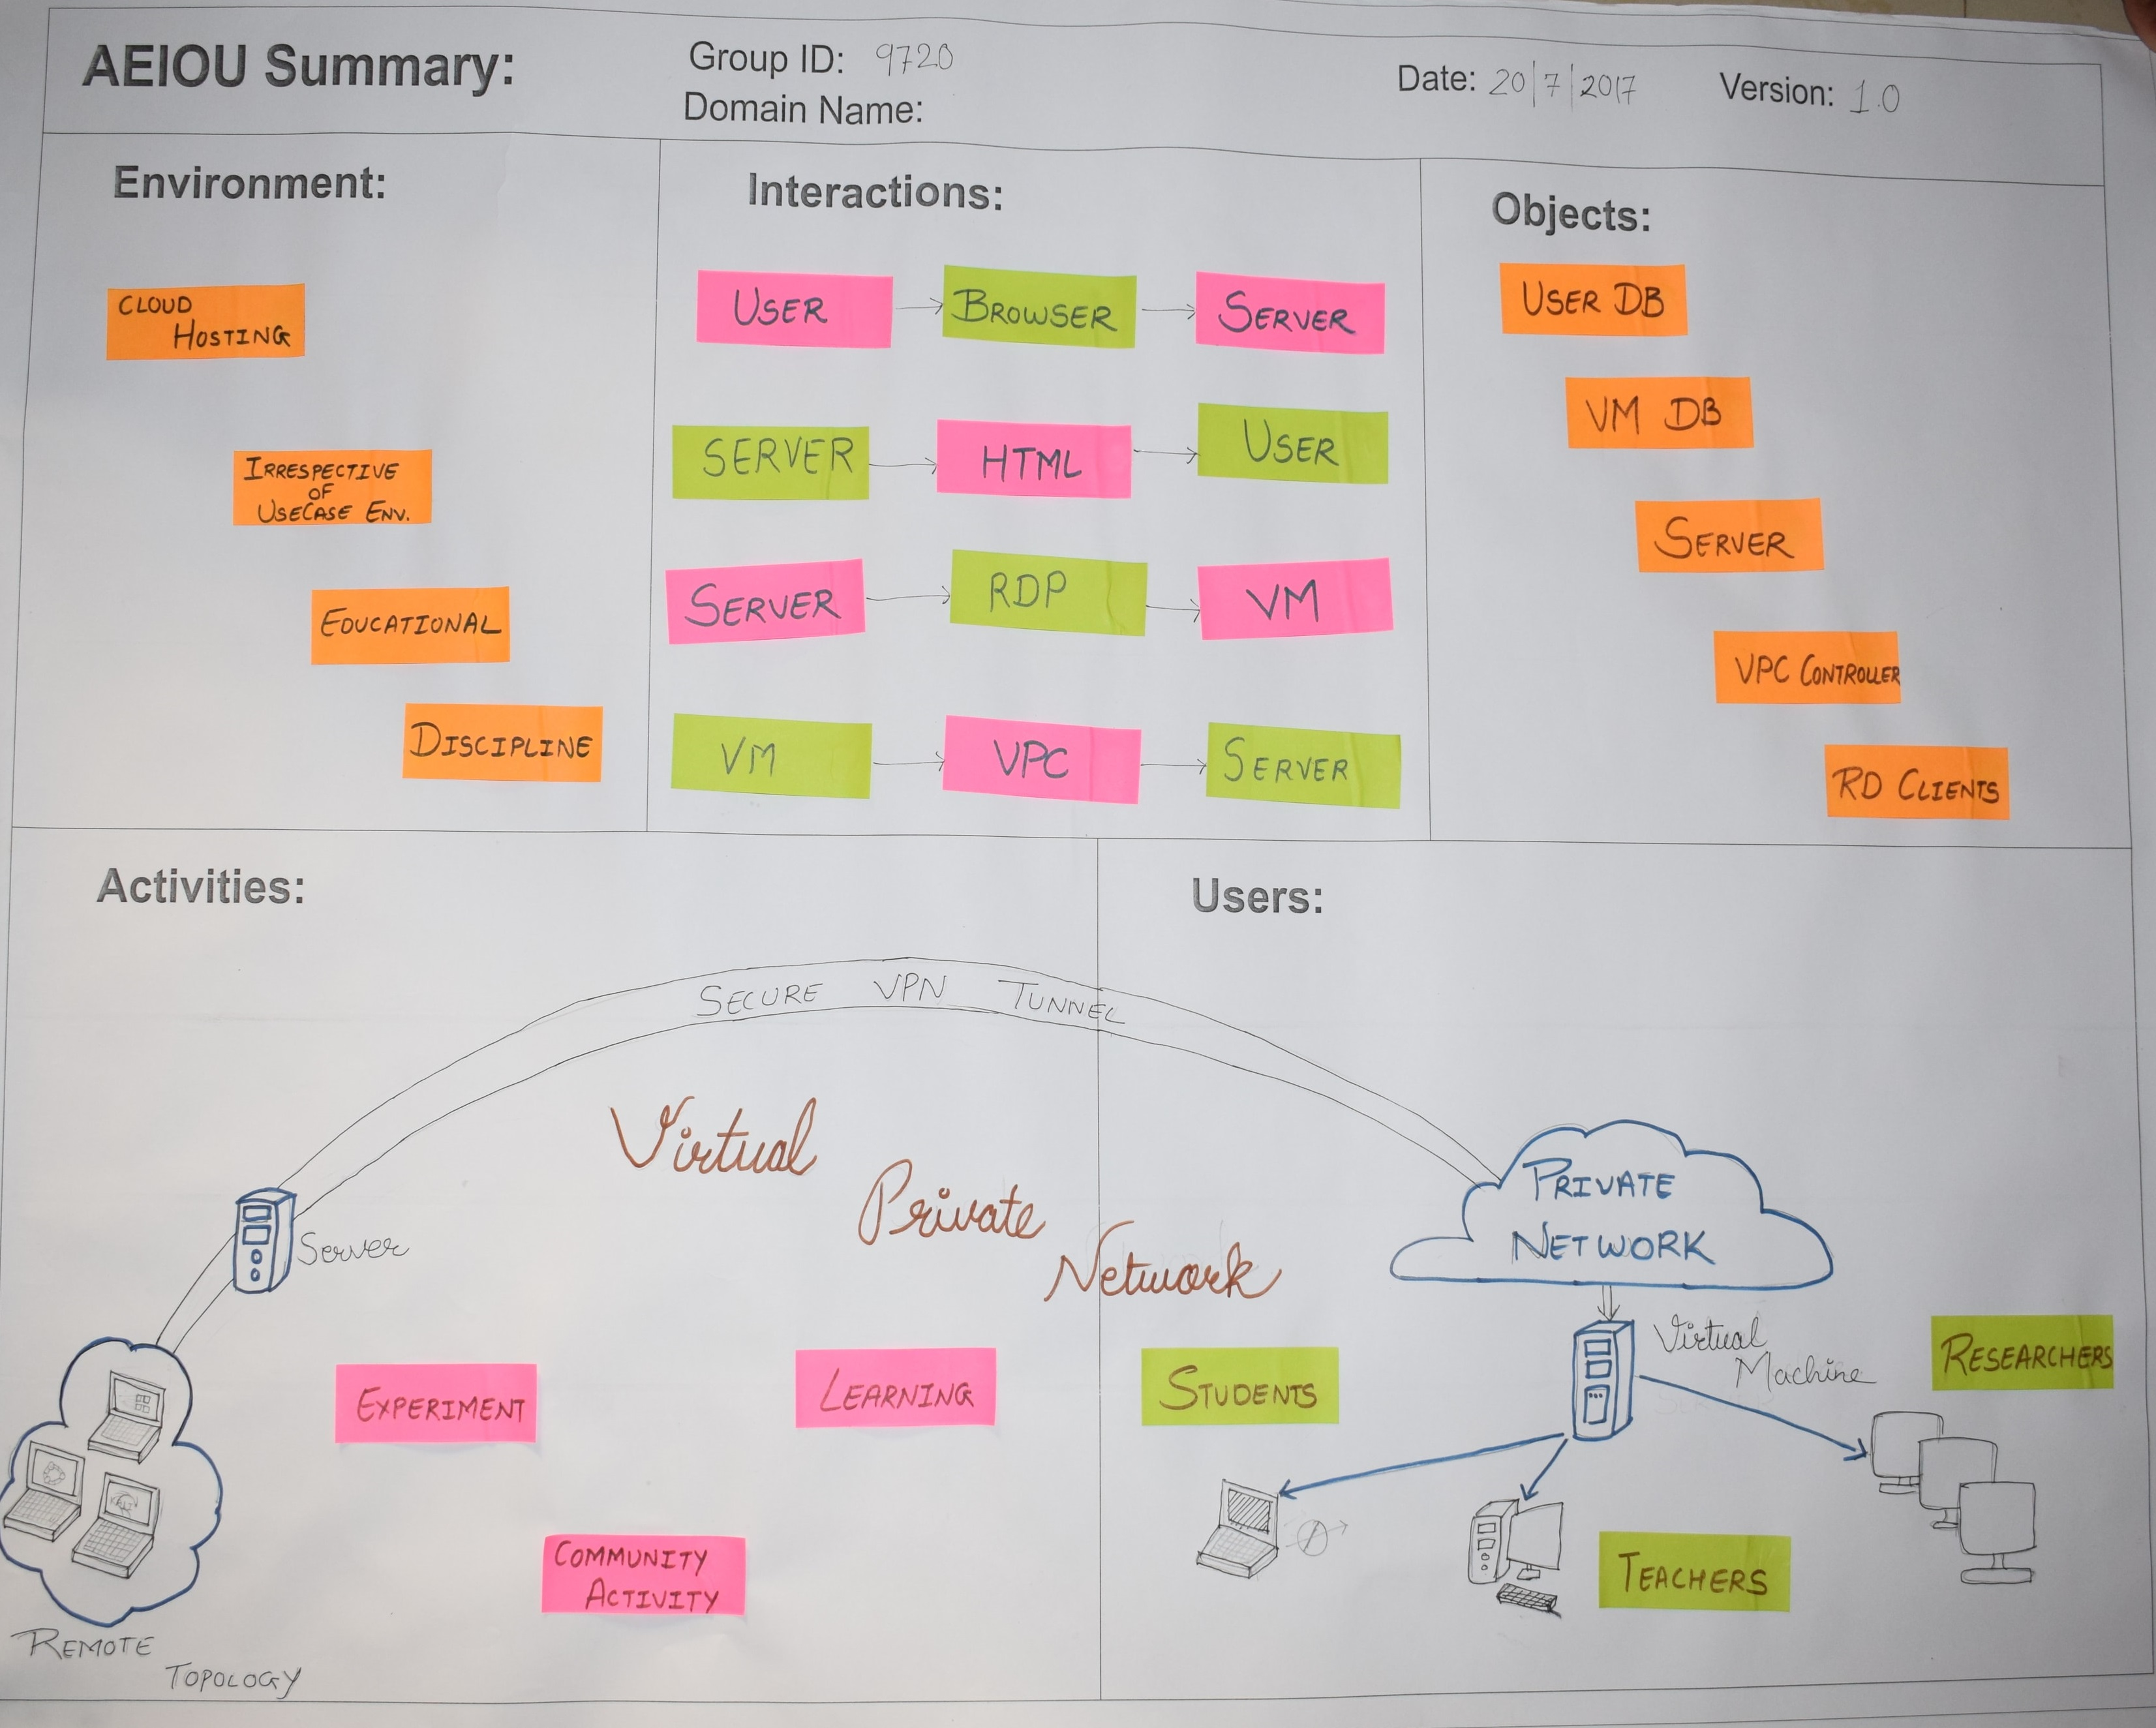
\includegraphics[width=0.685\linewidth,angle=0]{aeiou.jpg}
		\caption{AEIOU CANVAS }
	\end{figure}
	\subsection{Environment}
\textbf{}
 \flushleft The Environment which was observed was :
\begin{itemize}
\item Cloud hosting
\item Discipline 
\item Educational
\item Irrespective of Use case Environment 
\end{itemize}	
\subsection{Interaction}
\textbf{}
The Interaction takes place between 
\begin{enumerate}
\item User--Browser--Html--server
\item Server--html--user
\item Server--RDP--Vm
\item Vm--VPC--Server
\end{enumerate} 
\subsection{Object}
\textbf{}
The objects are 
\begin{enumerate}
\item User database
\item VM database
\item Server
\item VPC Control
\item RD Clients
\end{enumerate} 
\subsection{Activities}
\textbf{}
\begin{enumerate}
\item Experiment
\item Learning
\item Communicational Activity
\end{enumerate}
\subsection{Users}
\textbf{}
\begin{enumerate}
\item Students
\item teachers
\item researchers
\item Collaborators
\end{enumerate}
\newpage
	\section{Empathy Mapping} 
	\noindent\begin{figure}[h!]
		\centering
		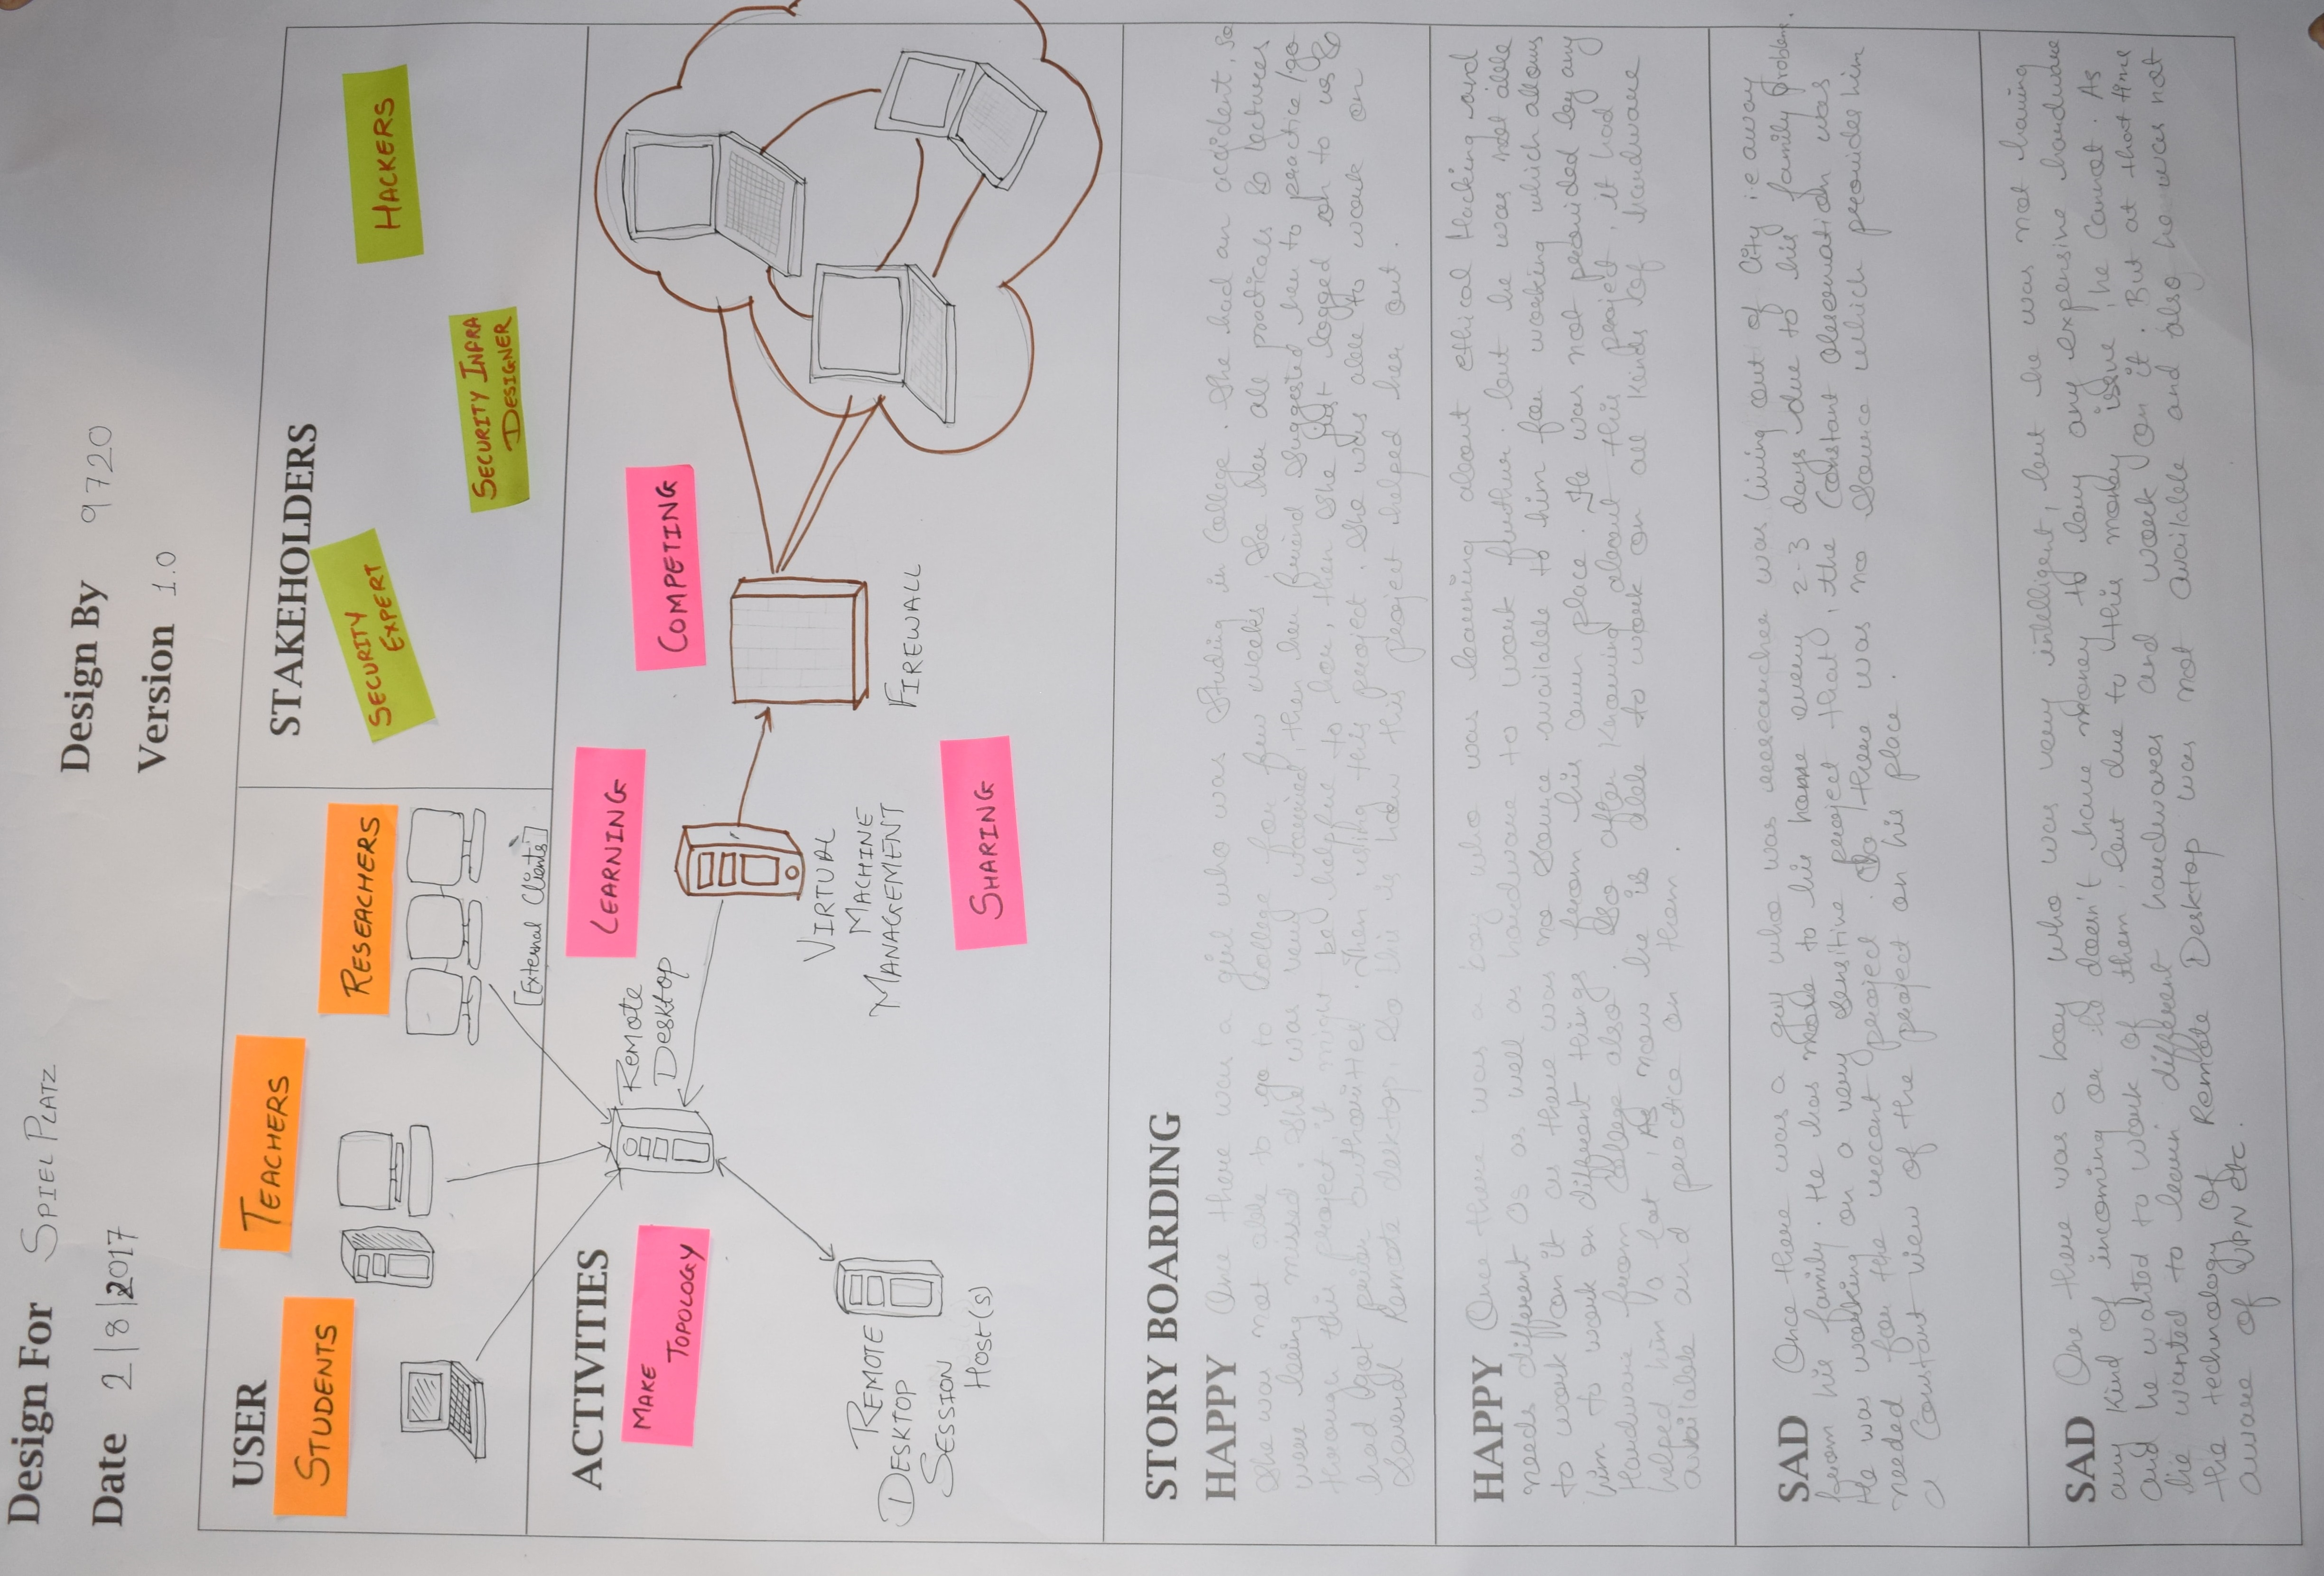
\includegraphics[width=0.685\linewidth,angle=0]{empathy.jpg}
		\caption{Empathy Mapping }
	\end{figure}
	\subsection{Users:}
	The user of our product will be : \\
	 \begin{itemize}
	\item Teachers
   \item Students 
   \item Researchers 
\end{itemize}
	\subsection{Stackholders:}
	\noindent\par The person or  the group of the people who are involved in this product are:\\
	\noindent 
	\noindent\textbf{}
	\begin{itemize}
	\item Security-Infrastructure-Designer
   \item Security-expert
   \item Hackers 
   	\end{itemize}
   	\subsection{Activity:}
	\noindent\par Activities mainly focuses on the key functions of the product.\\
	\noindent 
	\noindent\textbf{}
	\begin{itemize}
	\item Topology
   \item Share
   \item learn
   \item Collaborate
   	\end{itemize}
\newpage
\raggedright
	\section{Ideation Canvas}
	\begin{figure}[h!]
		\centering
		\includegraphics[width=1.0\linewidth,angle=0]
		{idea.jpg}
		\caption{Ideation Canvas}
		
	\end{figure}
	
	\subsection{People :}
	\textbf{}
	\begin{enumerate}
	\item Security Expert
	\item Ethical Hackers
	\item Security Infra Designer
	\item Students
	\item Teachers
	\item Reseachers	
	\end{enumerate}
	\subsection{Activities}
 \textbf{}
 The activities which are going to be undertaken by our project are:
	\begin{enumerate}
	\item Learning
	\item Sharing
	\item Topology
	\item Collaboration
	\end{enumerate}
	\subsection{Situation/Location/Context}
	The locations or the context on which our product will be useful are:
	\textbf{}
	\begin{enumerate}
	\item Practice-\&-Go
	\item Geo-Independent
	\item Any Device
	\item Anywhere
	\end{enumerate}
	\subsection{Props}
	\textbf{}
The props that will be used in our project are:
\begin{enumerate}
\item Laptop
\item Computer
\item Tablet
\item Server
\item Browser
\item ssh Clients
\end{enumerate}
\newpage
	\raggedright
	\section{Product Development Canvas}	
	\begin{figure}[h!]
		\centering
		\includegraphics[width=1.0\linewidth,angle=0]
		{pd.jpg}
		\caption{Product Development Canvas}
		
	\end{figure}
	\textbf{}
	\noindent \subsection{ Purpose:}
	The purpose behind doing this project and developing this product are as mentioned below:\\
	\textbf{}
	\begin{itemize}
	\item To make solution that have advantage of traditional method
	\end{itemize}
	\subsection{Product Experience}
	\begin{itemize}
	\item Easy
	\item Reliable
	\item Budget Friendly
	\item Accessible
	\end{itemize}
	\subsubsection{Product Function}
	\begin{enumerate}
	\item Remote Topology for Practice
	\item Geo-Independent
	\end{enumerate}
\subsubsection{Product Features}
\begin{itemize}
\item cost-friendly
\item scalable 
\item collaboration
\item Access-on-go
\end{itemize}
\newpage
\chapter{Implementation}
\section{Diagram}
\subsubsection{Class Diagram :}
\begin{figure}
\centering
\includegraphics[totalheight=0.5\textheight,angle=0]		{Class.jpg}
		\caption{Class Diagram}
\end{figure}
	\subsubsection{Sequence Diagram :}
	\begin{figure}
		\centering	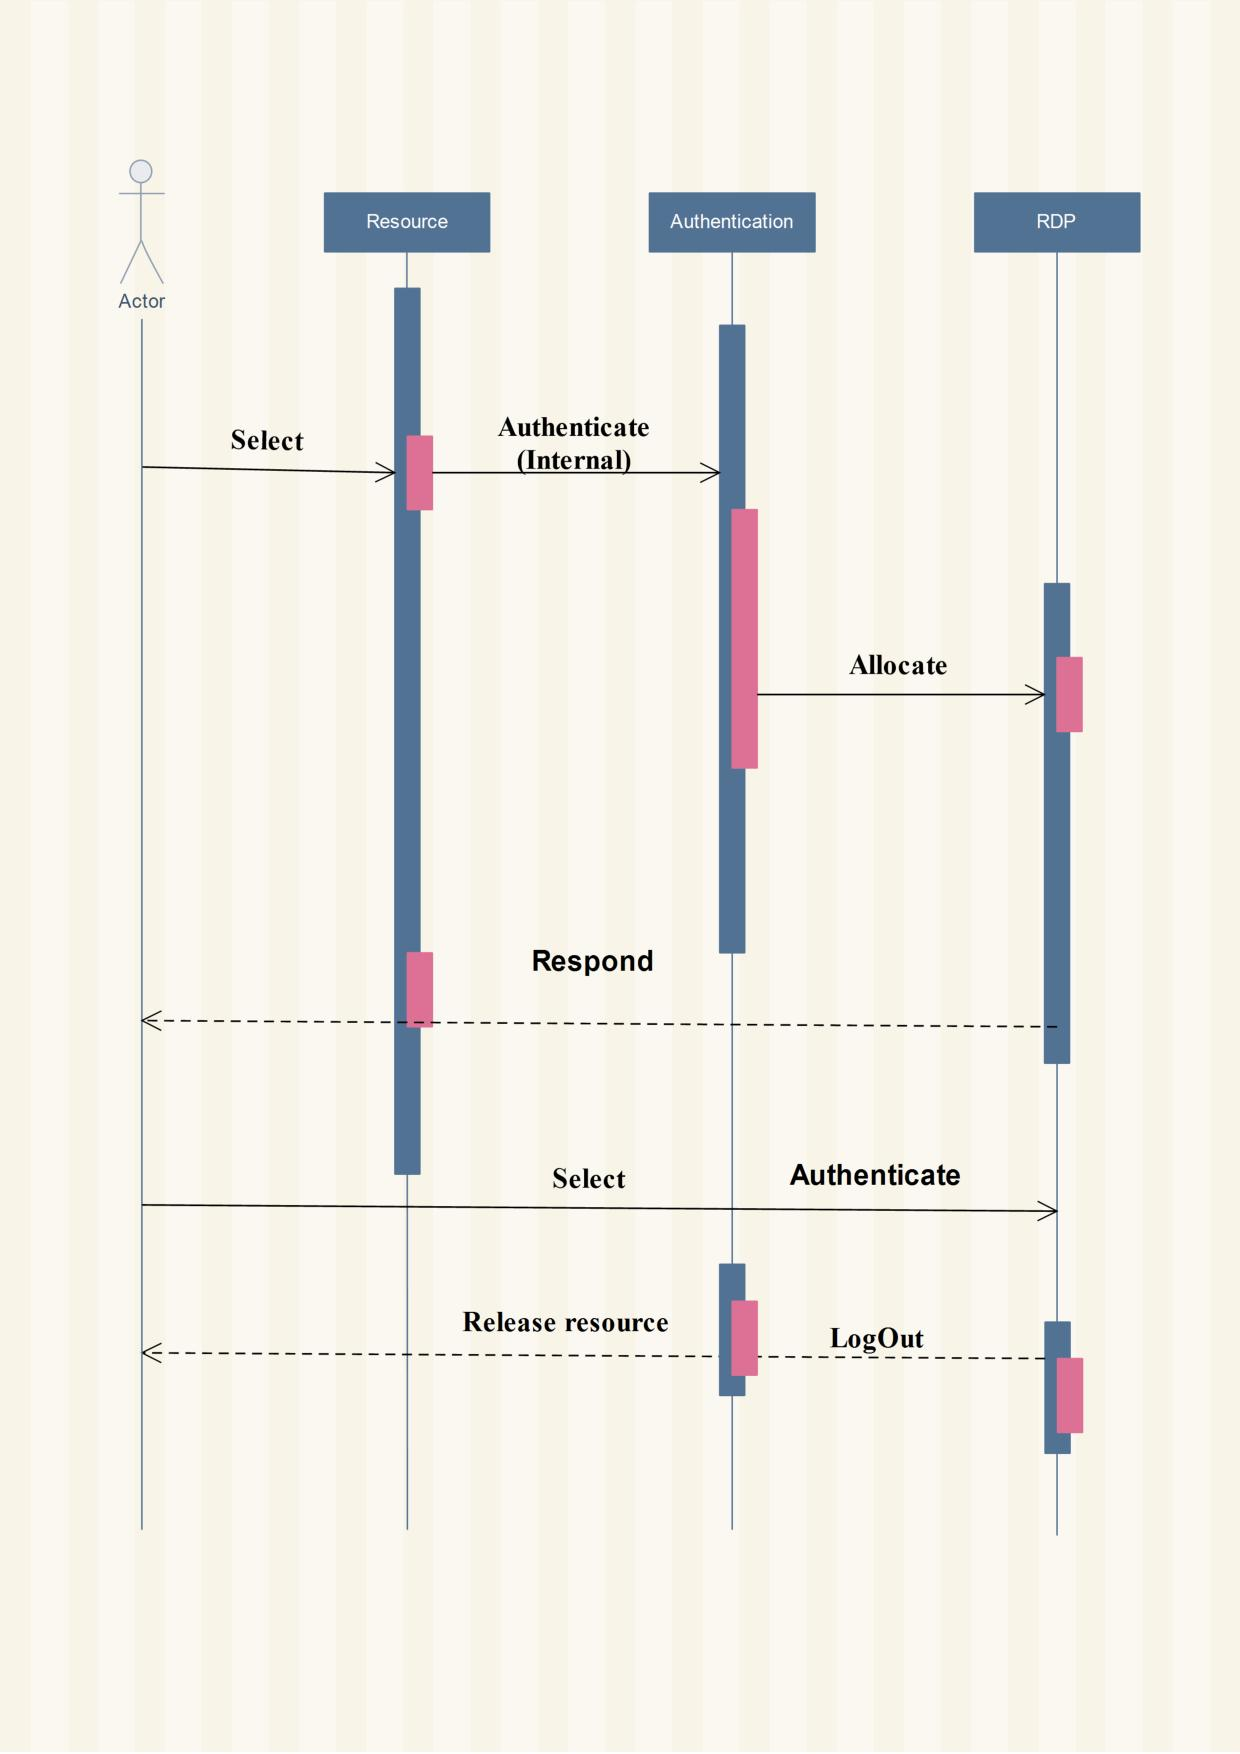
\includegraphics[width=1.0\linewidth,angle=0]
		{seq2.jpg}
		\caption{Sequence Diagram}
	\end{figure}
	\begin{figure}
		\centering \vfill	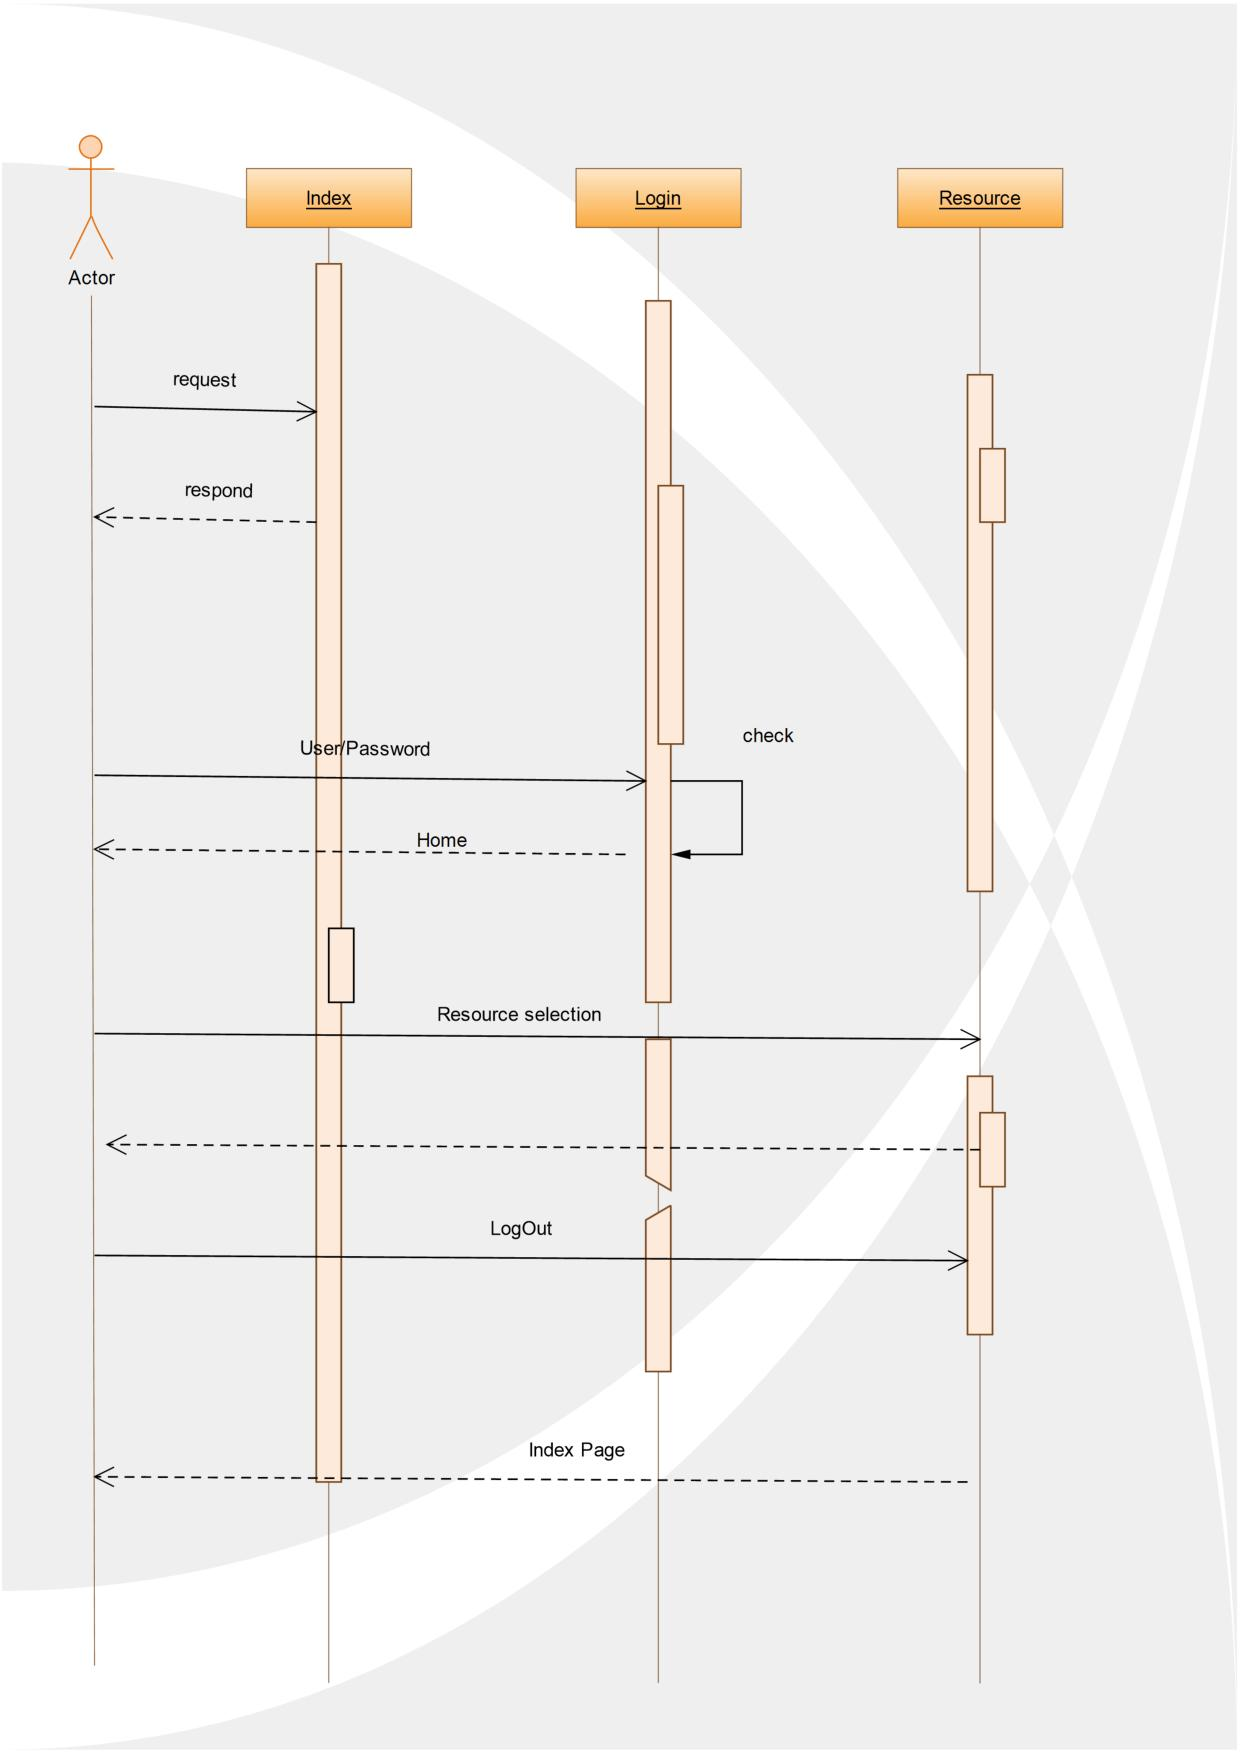
\includegraphics[totalheight=0.5\textheight,angle=0]
		{seq1.jpg}
		\caption{Sequence Diagram}
	\end{figure}
	\subsubsection{Entity Relation Diagram :}
%\begin{figure} \centering	\includegraphics[width=1.0\linewidth,angle=0]{ER.jpg}
%	\caption{Entity relation Diagram}
%	\end{figure}
	\subsubsection{Activity Diagram :}
\begin{figure}
		\centering	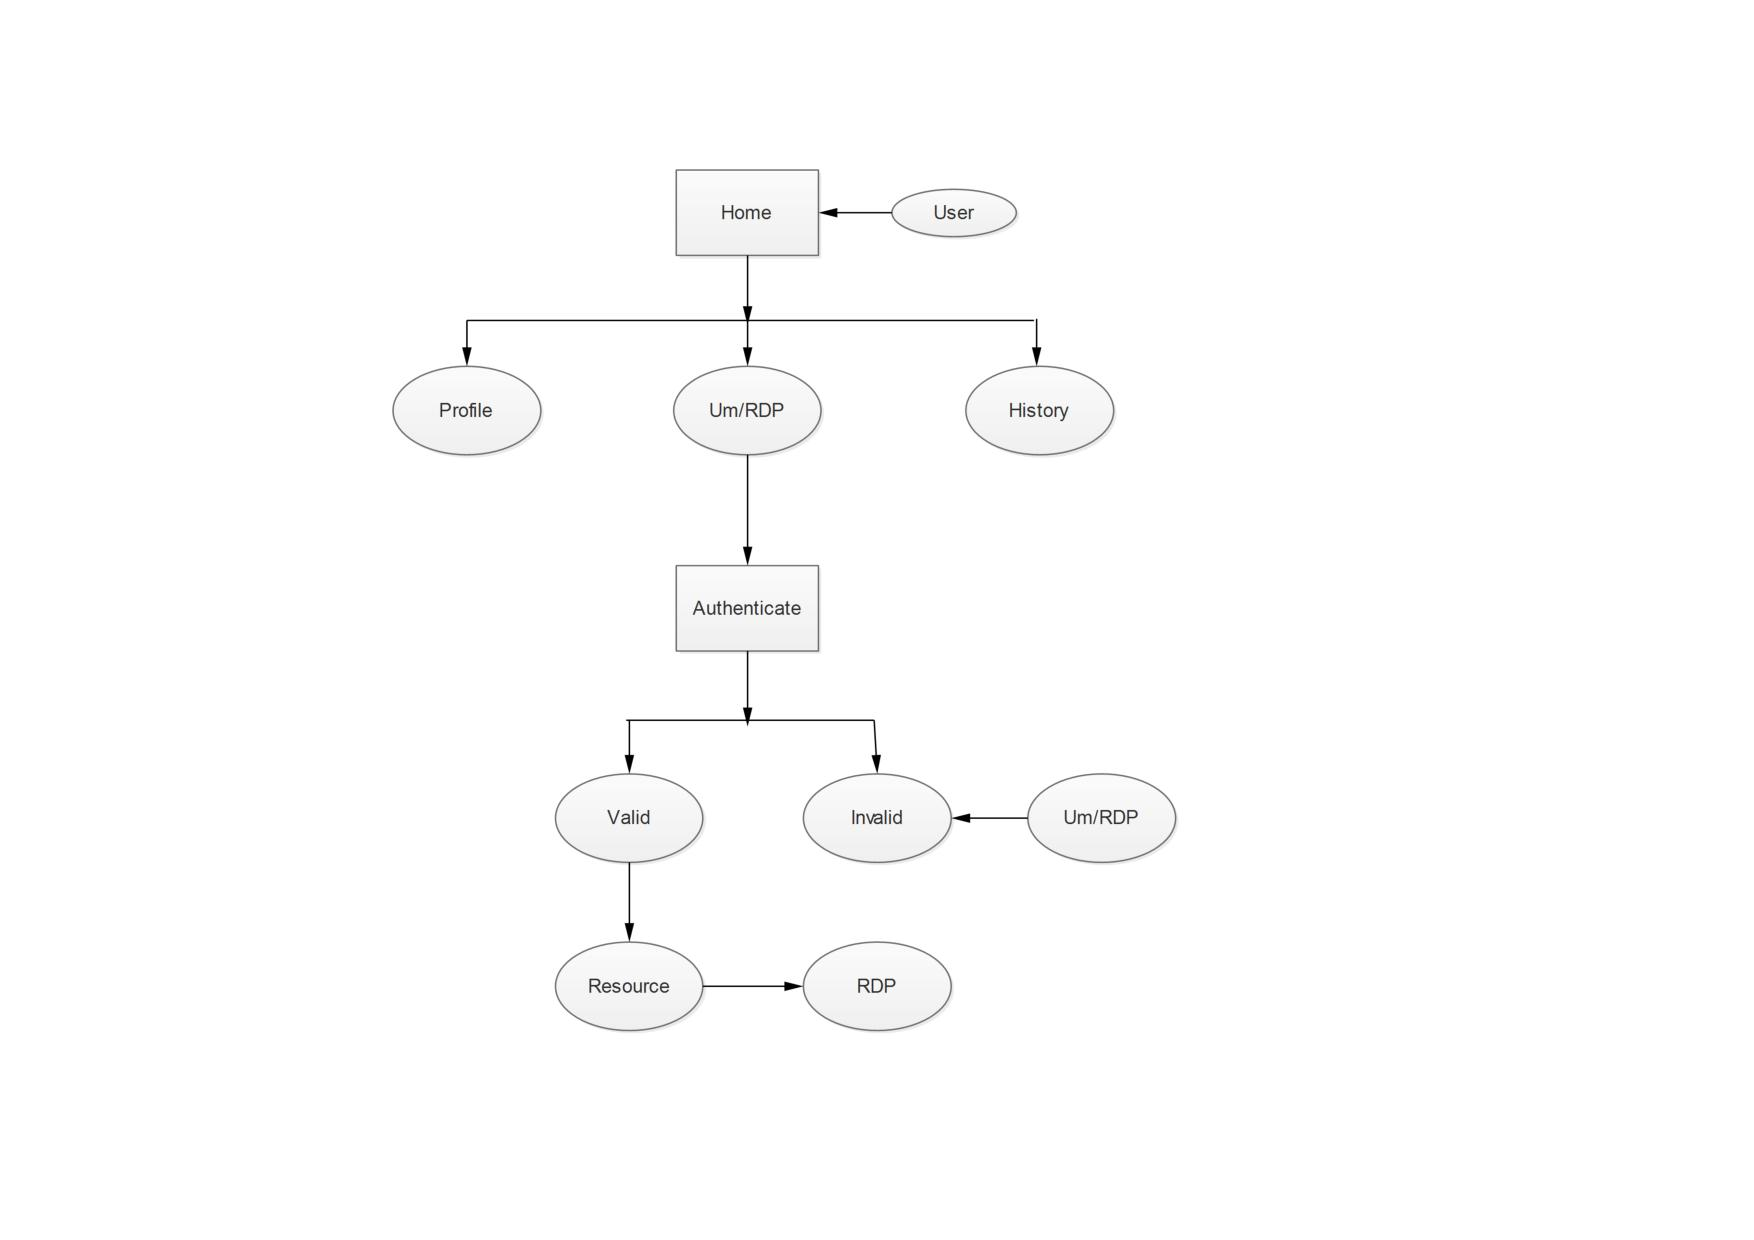
\includegraphics[width=1.0\linewidth,angle=0]
		{activity1.jpg}
		\caption{Activity Diagram}
	\end{figure}
	\begin{figure}
		\centering	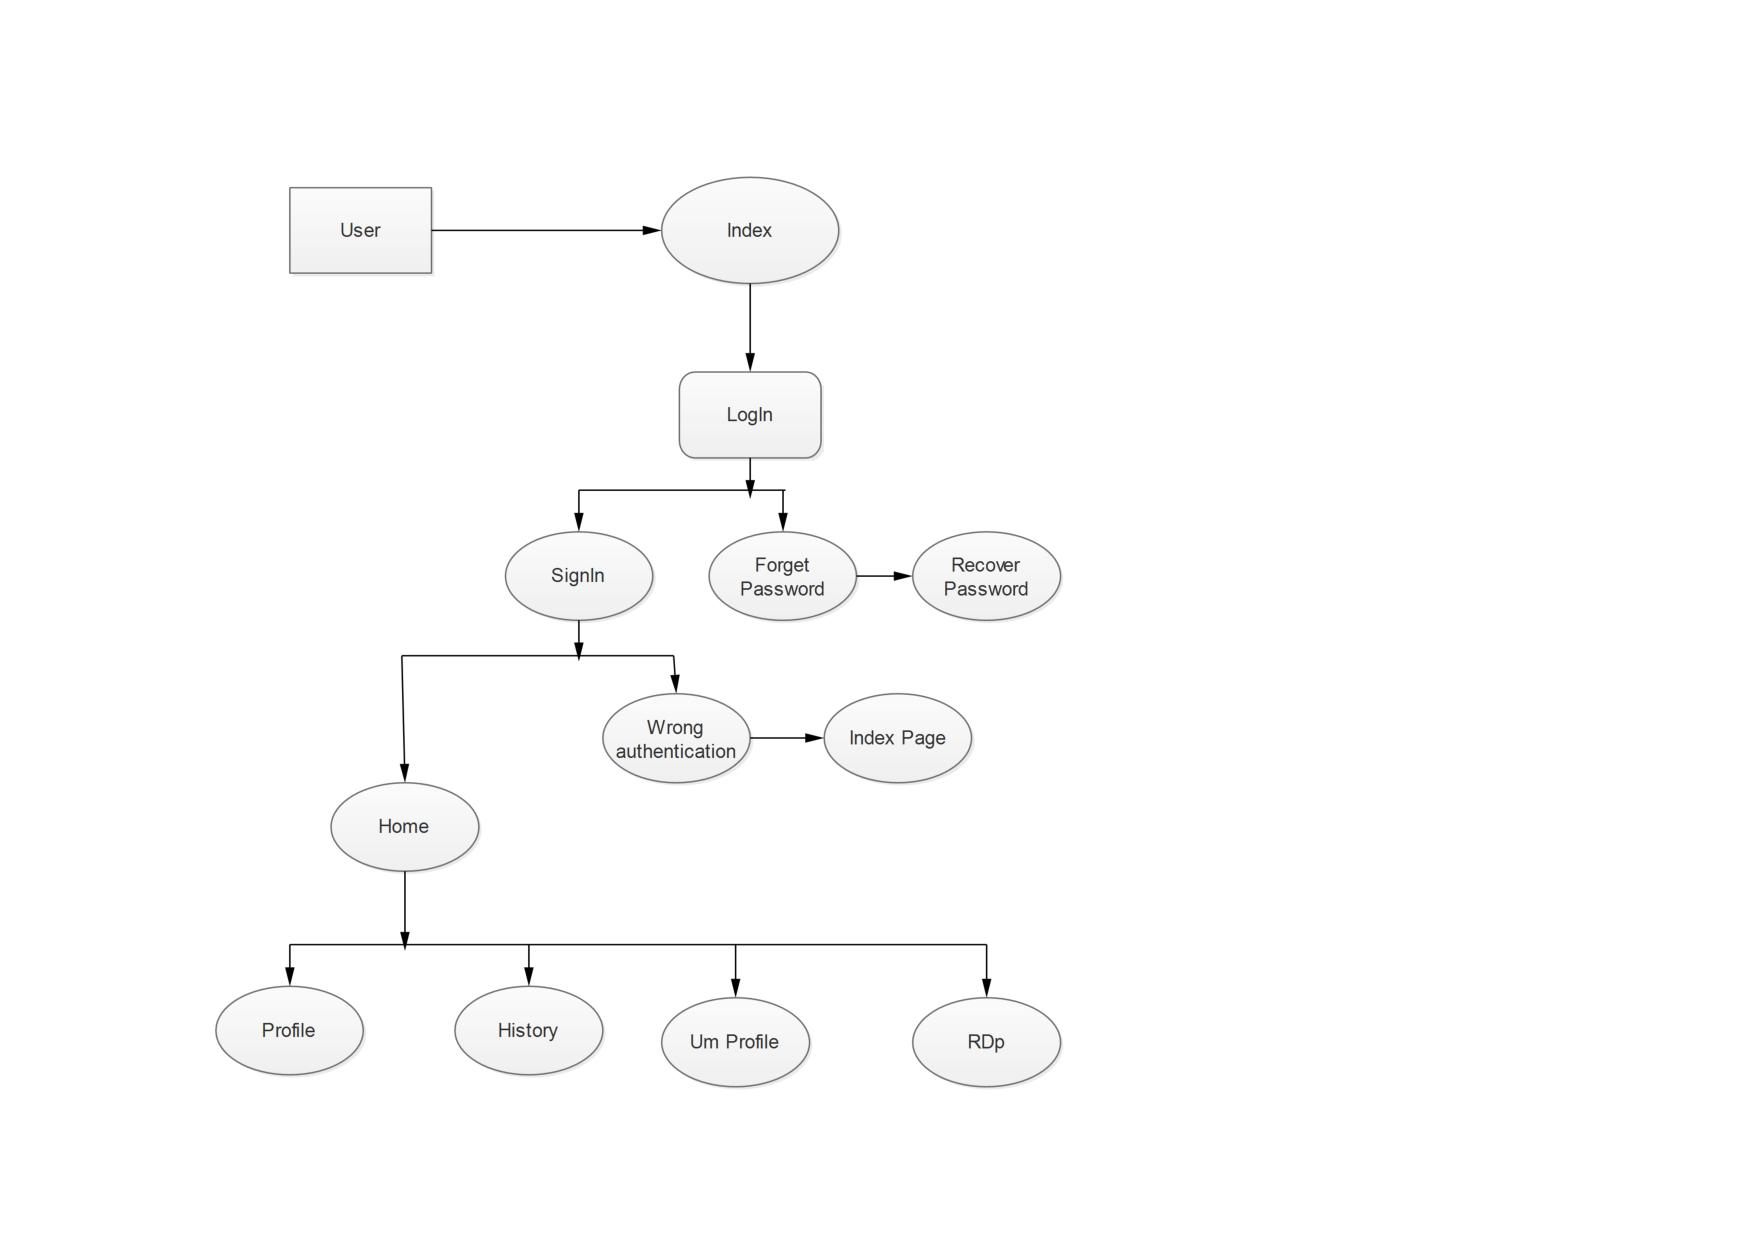
\includegraphics[width=1.0\linewidth,angle=0]
		{activity2.jpg}
		\caption{Activity Diagram}
	\end{figure}
	\subsubsection{Use Case Diagram :}
\begin{figure}
\centering
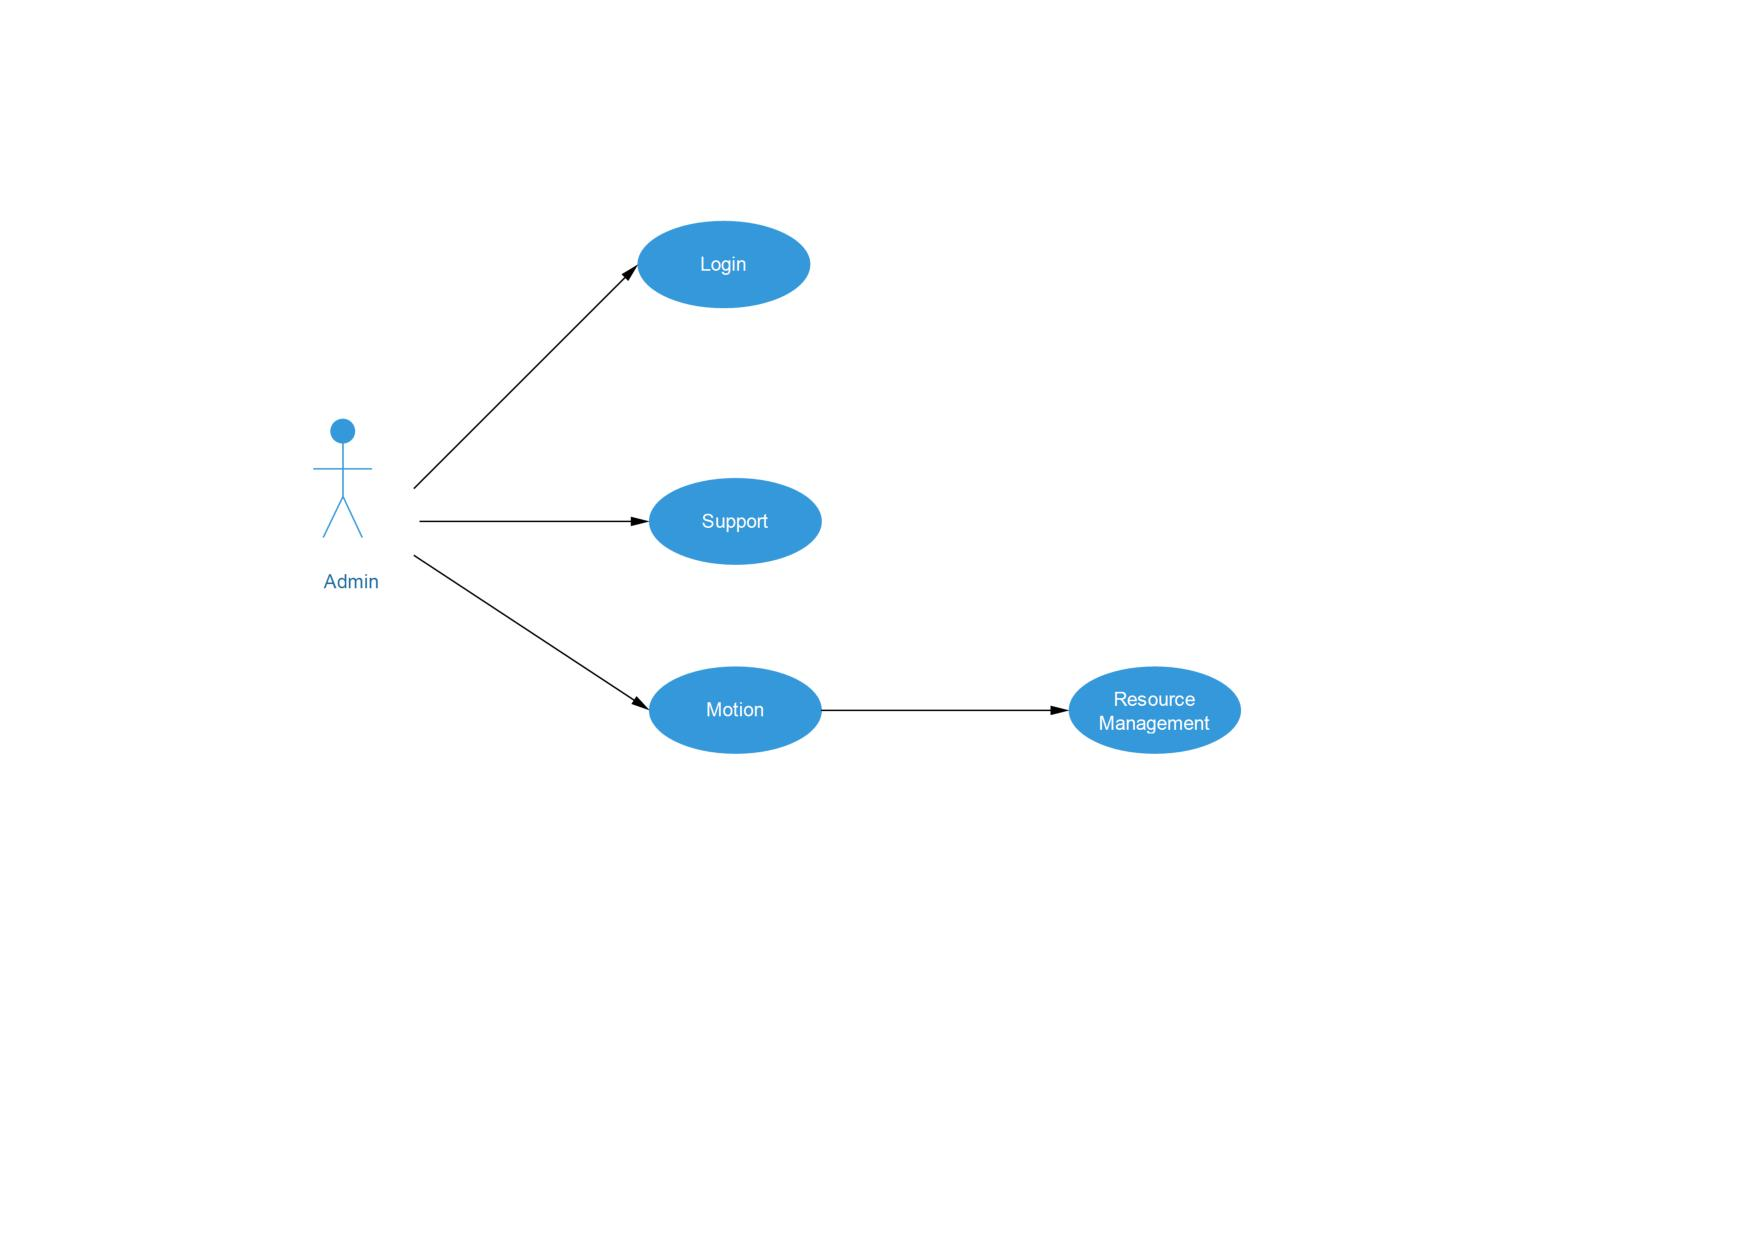
\includegraphics[height=5cm]{use1.jpg}
\caption{Usecase Diagram}
\end{figure}
\begin{figure}
		\centering	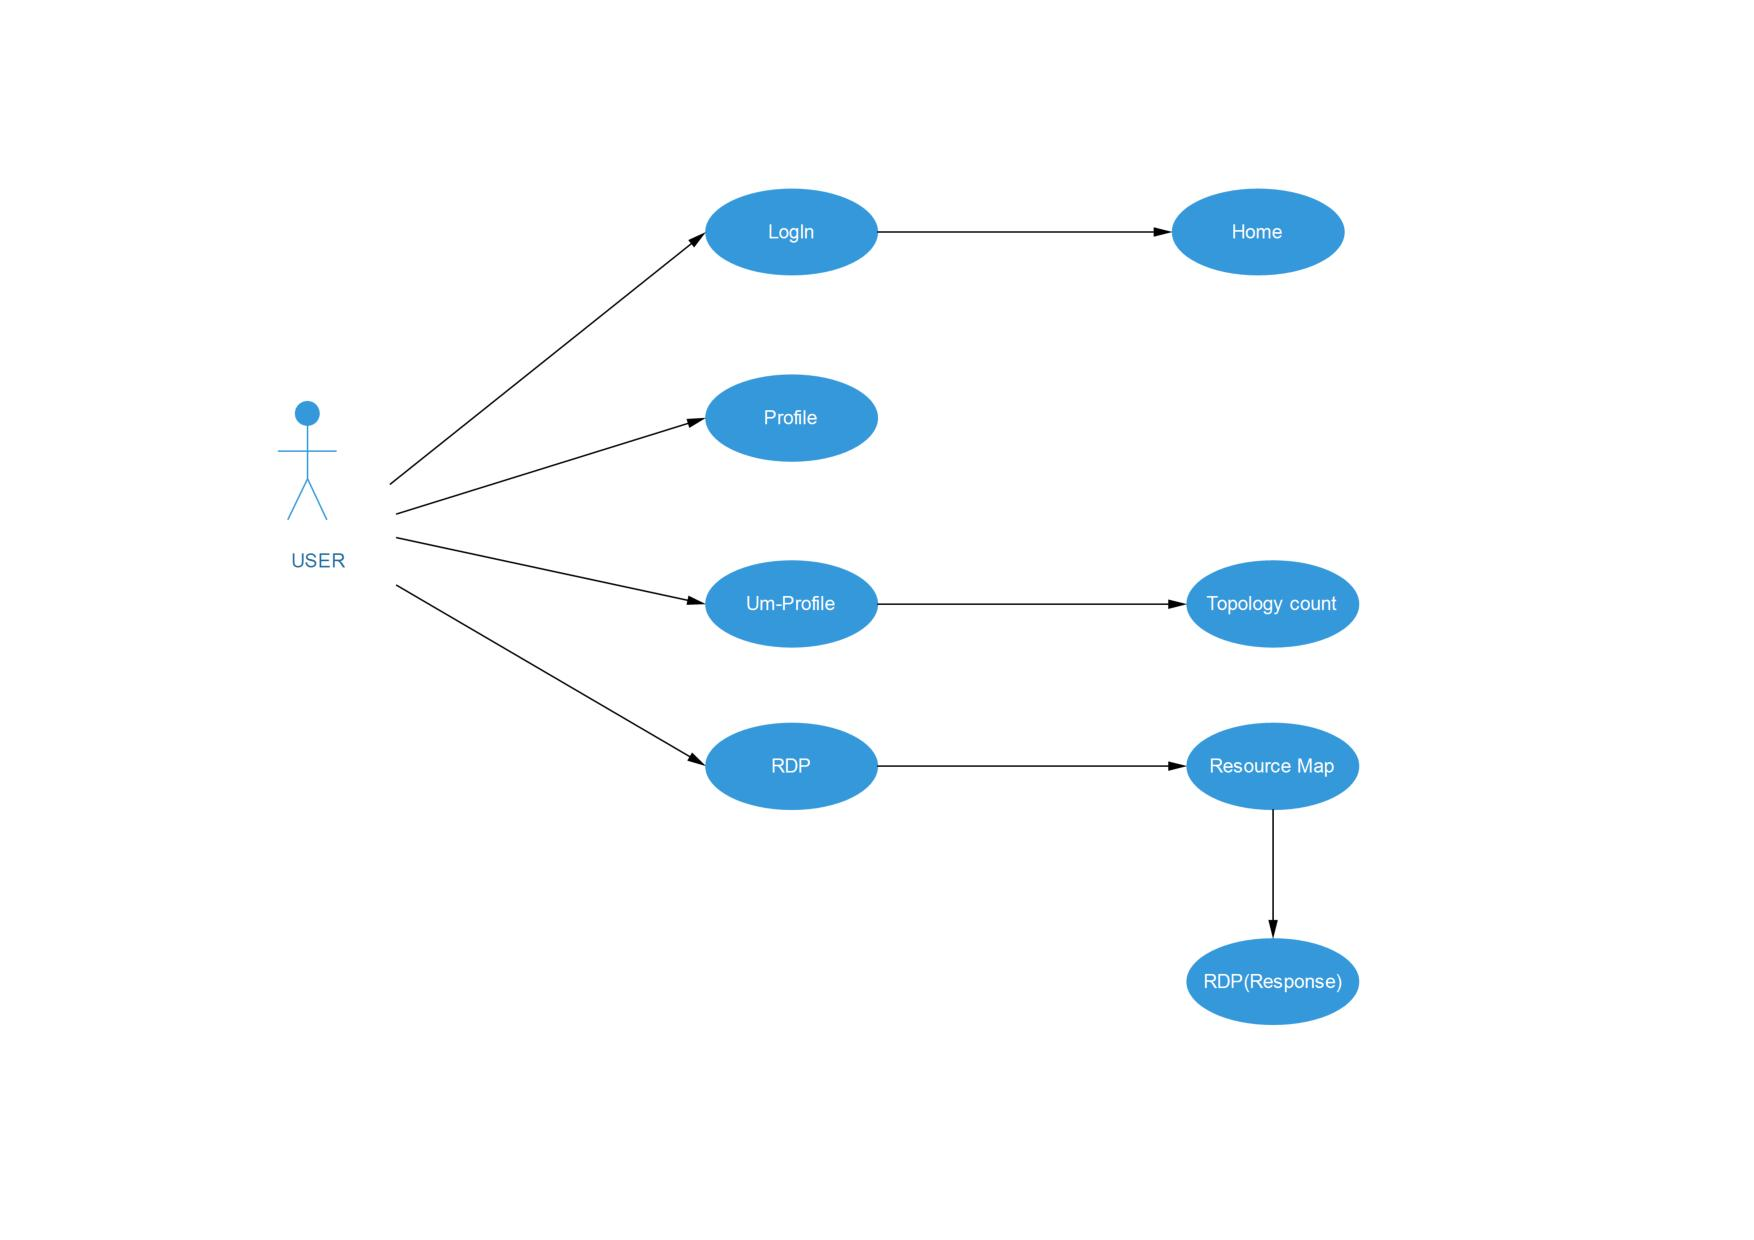
\includegraphics[width=1.0\linewidth,angle=0]
		{use2.jpg}
		\caption{Usecase Diagram}
	\end{figure}
	\newpage
\section{Designing }
\section{Hardware Implementation}
As soon as the Request \& Authentication id done successfully the resource is available to the end user and the under explanation is more precise . 
\subsubsection{Hardware Connections}
\noindent\begin{figure}[h!]
		\centering
		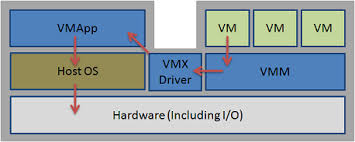
\includegraphics[width=0.685\linewidth,angle=0]{vm.jpg}
		\caption{Diagram }
	\end{figure}
\noindent\begin{figure}[h!]
		\centering
		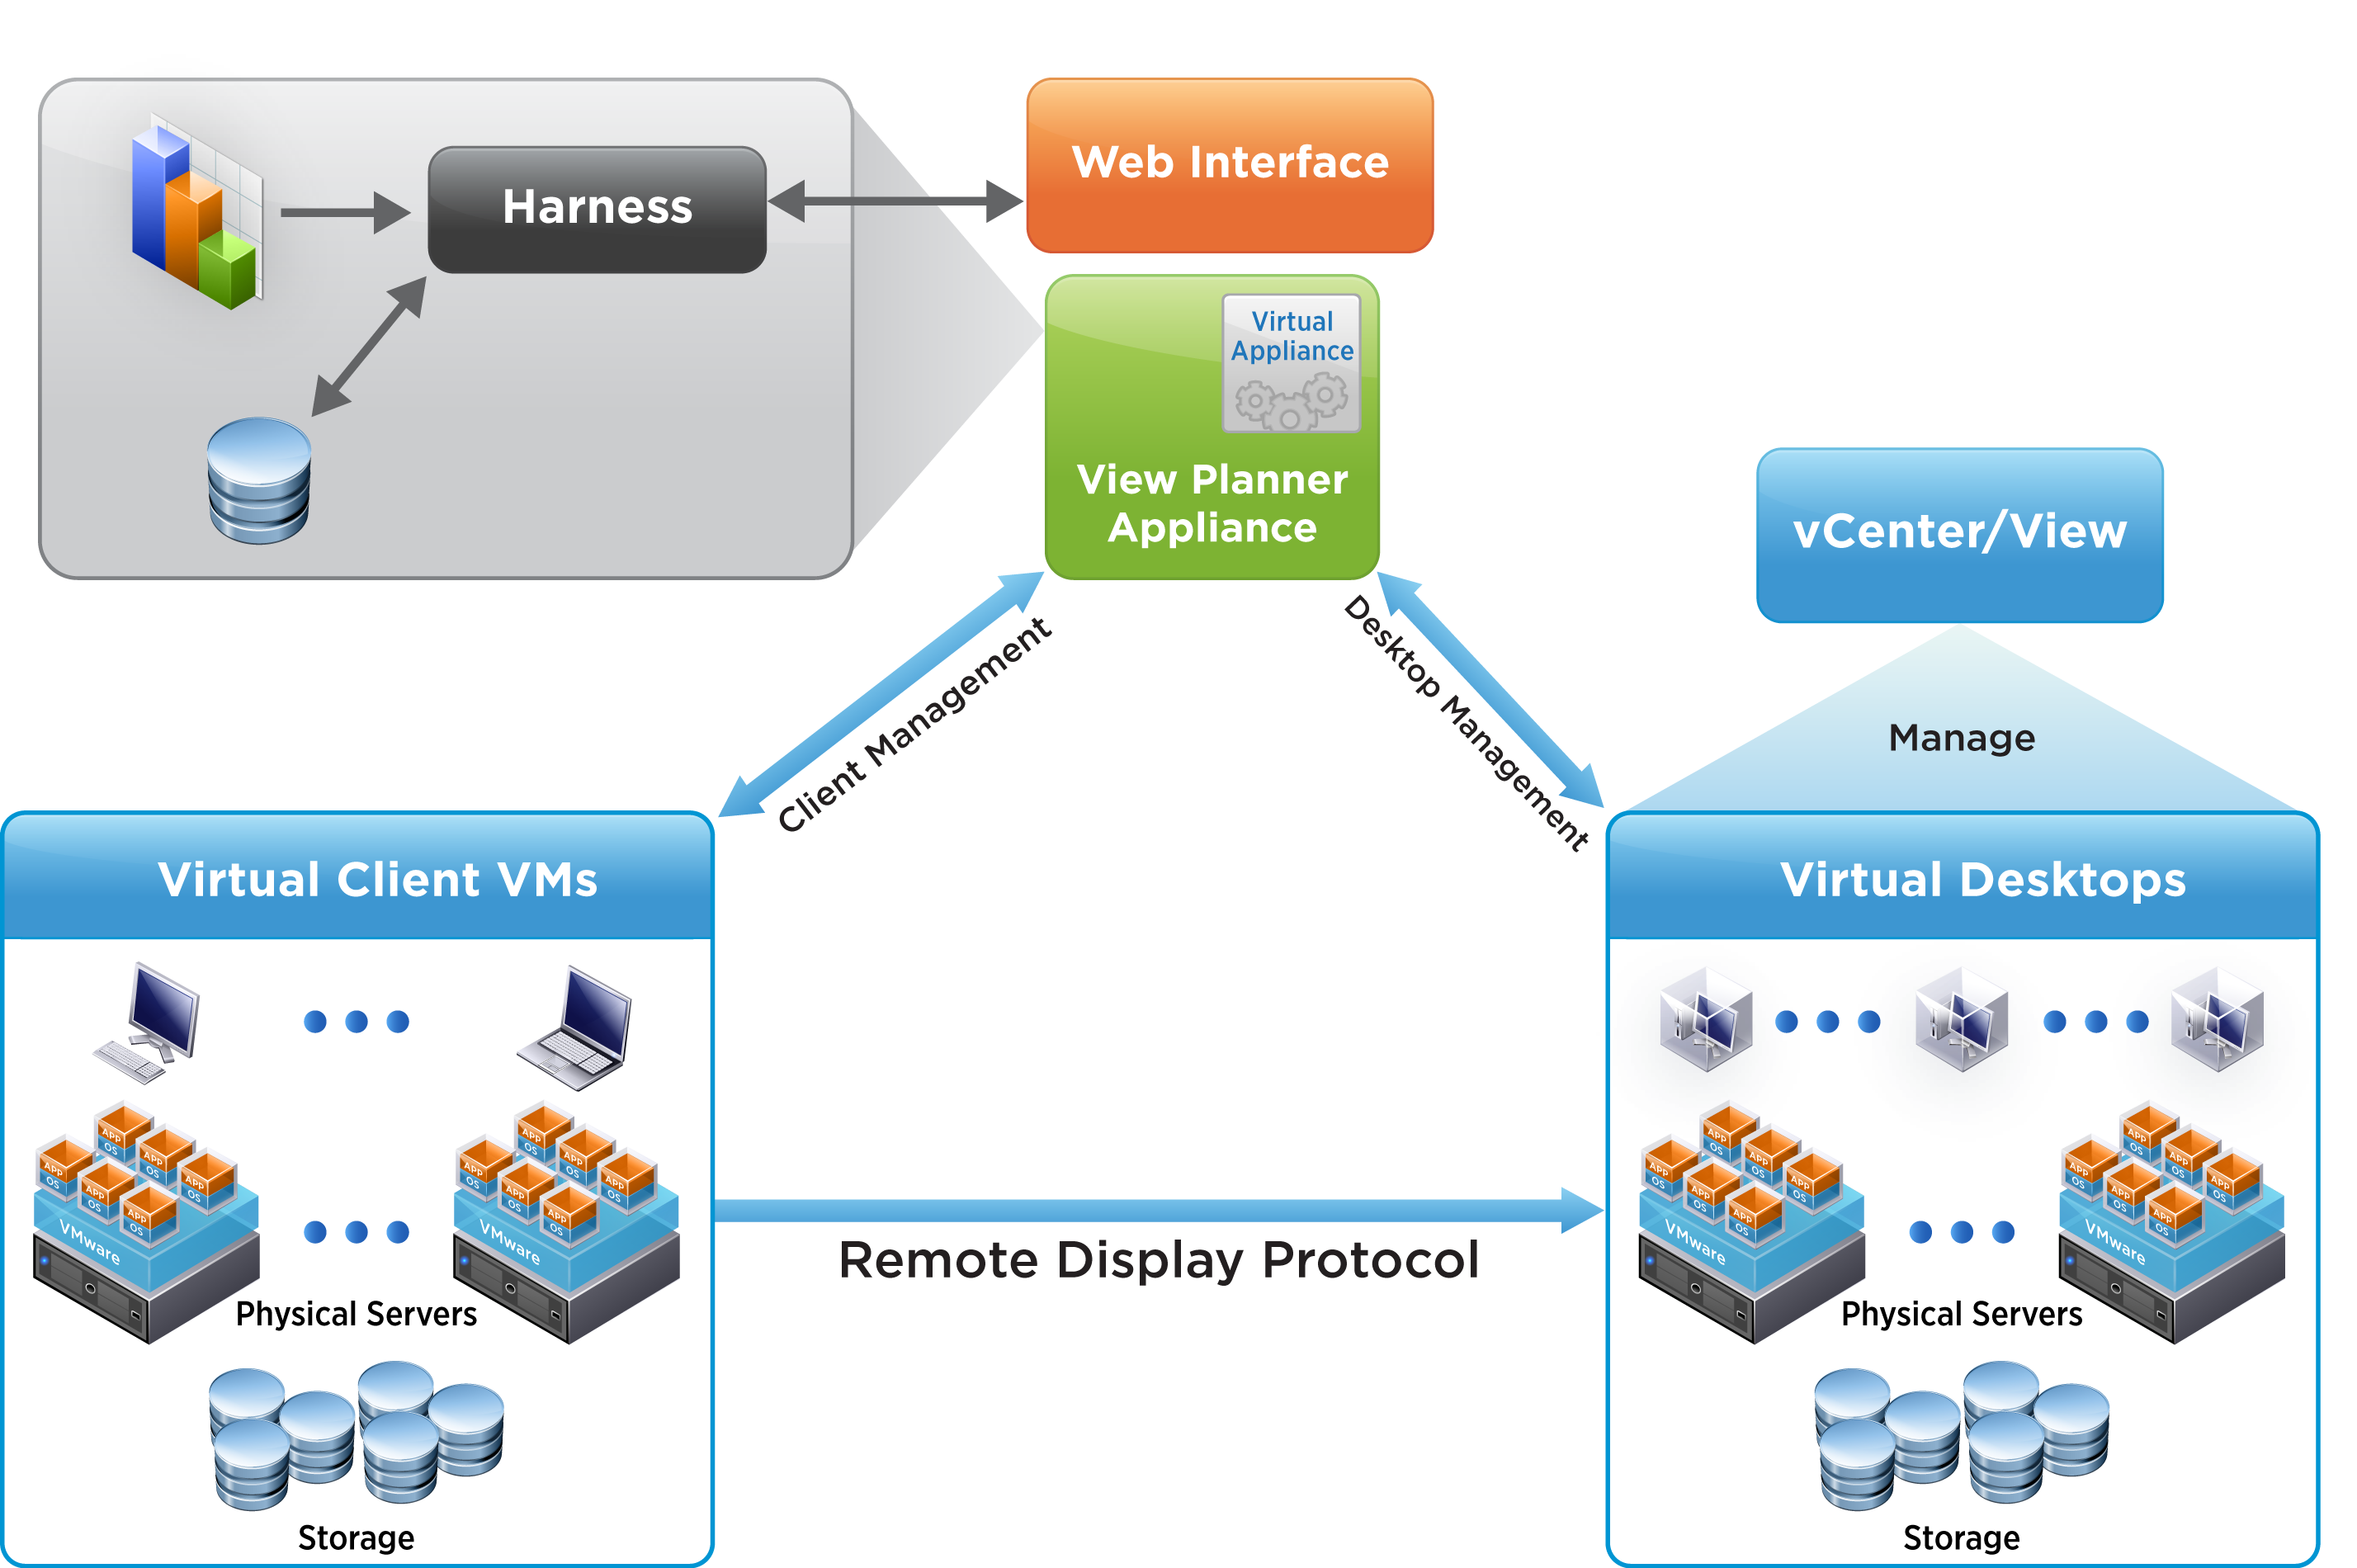
\includegraphics[width=0.685\linewidth,angle=0]{v.png}
		\caption{Diagram }
	\end{figure}	
	\noindent\begin{figure}[h!]
		\centering
	%	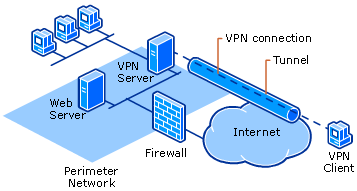
\includegraphics[width=0.685\linewidth,angle=0]{vpn.jpg}
		\caption{Figure }
	\end{figure}
\newpage
\chapter{Advantages and Features}
\section{Advantages of our Work}
\begin{enumerate}
\item A secure space to practice Cyber attacks
\item A virtual Platform to learn , share and community
\item Scalable , 
\item traceable and all tools at one place
\end{enumerate}
\section{Usefulness with respect to existing solutions }
\begin{enumerate}
\item Affordable price and hands on equipments 
\item Accessible from any where and on any platform
\end{enumerate}
\section{Unique Features}
\begin{enumerate}
\item The impact of the Cyber attack and practice will be walled under the cloud infrastructure \& simulation.
\item Law can be maintain and the practice is Ethical.
\end{enumerate}
\section{Future Scope}
\begin{enumerate}
\item Development \& User interface Alternative
\item Inter-networking Improvement \& more Hardware Support
\item Business \& Start up Back bone
\end{enumerate}
\chapter{Conclusion}
The virtual environment for Practising cyber security is indeed not only to the cyber security experts it will also be use full for the students , professional \& the institution which are preparing the next worriers . Our Solution SpielPlatz 	includes the creation of labs , sharing of  expensive hardware and tools . This lab not only focus on practical hands on practice but also on theoretical concepts and  discussion  This lab is based on cloud arch and available over 	internet using just a web browser.This lab also provide the GUI \& SSH 	connectivity over web and the lab is compatible with any device which has a HTML5 supported web browser and a internet connection. There is one more concert that the security of the cyber attack or practice should be walled inside the cloud practice environment.
\chapter{Reference}
https://docs.oracle.com/javase/tutorial/
https://guacamole.incubator.apache.org/
http://tomcat.apache.org/tomcat-8.5-doc/index.html
https://www.tutorialspoint.com/unix/
https://msdn.microsoft.com/en-us/library/cc240445.aspx
https://tools.ietf.org/html/rfc6143
https://guacamole.incubator.apache.org/api-documentation/
\end{document}